\chapter{Painel Solar} \label{secao:painel solar}

\section{Introdução}

Este capítulo apresentará uma breve introdução sobre o funcionamento de células solares, explicando o efeito fotovoltaico, seguido de um circuito equivalente utilizado para modelar um painel real, e, por fim, algoritmos utilizados para operar os painéis sempre com máxima eficiência.

\section{Como Funcionam as Células Solares}

O funcionamento de células solares é baseado no efeito fotovoltaico, ou seja, a geração de tensão ou corrente elétrica a partir da incidência de luz. O efeito fotovoltaico ocorre da seguinte maneira: em um semicondutor ideal existem dois níveis de energia que elétrons podem ser excitados, representados pela camada de valência, com energia baixa, e a camada de condução, com energia mais alta. Entre estas duas camadas existe o chamado \textit{bandgap}, uma região com níveis de energia que os elétrons não podem assumir. Quando um fóton entra em contato com o semicondutor os elétrons na camada de valência absorvem sua energia e passam para a camada de condução, gerando uma corrente elétrica. Como não é possível que os elétrons possuam níveis intermediários de energia fótons que não possuam energia superior ao \textit{bandgap} não são absorvidos e passam sem interagir com a célula.\cite{jager2014}.

\section{Circuito Equivalente de um Painel Solar}

Em uma célula real existem perdas causadas por aquecimento no movimento dos elétrons, por impurezas no material que geram novos níveis de energia dentro do \textit{bandgap} e também por recombinação na junção p-n \cite{blakers2013}. Portanto para representar as células solares através de um circuito equivalente é necessário uma fonte de corrente associada com alguns componentes que representam as perdas.

O modelo para uma célula aqui utilizado é apresentado em \cite{erdem2013}. O circuito equivalente é composto por uma fonte de corrente \gls{Iph}, um diodo D, uma resistência paralela \gls{Rp} e uma resistência série \gls{Rs}. Este circuito pode ser visto na Figura \ref{modelo_celula_solar}, onde \gls{Iph} é a corrente fotogerada do painel, \gls{ID} é a corrente do diodo, \gls{IRp} é a corrente na resistência paralela, \gls{I} é a corrente da célula e \gls{V} é a tensão da célula.

\begin{figure}[!htpb]
\begin{center}
\begin{circuitikz} [american]
\draw
(0,0) to[I, l = I\textsubscript{ph}] (0,3) -- (2,3)
      to[diode, l = D] (2,0) -- (0,0)
(2,3) to[short] (4,3)
(4,3) to[resistor, l = R\textsubscript{p}] (4,0) -- (2,0)
(4,3) to [short] (4.5,3)
(4.5,3) to[resistor, l = R\textsubscript{s}] (6.5,3)
	  to[short, -o] (7,3)
(4,0) to[short, -o] (7,0)
(7,3) to[open, v=V] (7,0);
\draw[->] (6.25, 3.25) -- (7,3.25) node[midway, above] {I};
\draw[->] (2.25, 2.75) -- (2.25, 2) node[midway, right] {I\textsubscript{D}};
\draw[->] (4.25, 2.75) -- (4.25, 2) node[midway, right] {I\textsubscript{R\textsubscript{p}}};
\end{circuitikz}
\end{center}
\caption{Circuito equivalente da célula solar}
\label{modelo_celula_solar}
\end{figure}

A partir da análise do circuito equivalente, temos a seguinte relação entre a corrente e a tensão da célula:

\begin{equation} \label{eq:relacao_corrente_tensao_celula}
I = I_{ph} - I_{D} - I_{R_{p}}
\end{equation}

Por simplicidade e sem perda de precisão \gls{Iph} pode ser determinada diretamente pela corrente de curto-circuito \gls{Isc} do painel, respeitando-se a dependência com a irradiância \gls{E} e a temperatura da célula \gls{Tc} (equação \ref{eq:corrente_fotogerada}), assim pode-se obtê-la diretamente dos \textit{datasheets} fornecidos pelos fabricantes. 

\begin{equation} \label{eq:corrente_fotogerada}
I_{ph} = I_{sc}\cdot \frac{E}{E_{0}} \cdot [1 + \Delta_{I_{sc}}(T_{c} - T_{0})]
\end{equation}

A corrente no diodo é dada pela equação \ref{eq:corrente_diodo}, onde \gls{Io} é a corrente de saturação quando não há iluminação sobre a célula, \gls{q} é a carga de um elétron, \gls{n} é o fator de idealidade, \gls{k} é a constante de Boltzmann e \gls{Tc} é a temperatura da célula \cite{bellia2014}.

\begin{equation} \label{eq:corrente_diodo}
I_{D} = I_{o}(e^{-\frac{q(V+I\cdot R_{s})}{nkT_{c}}}-1)
\end{equation}

A corrente no resistor \gls{Rp} pode ser obtida através da equação \ref{eq:corrente_Rp}, conhecida como Lei de Ohm.

\begin{equation} \label{eq:corrente_Rp}
I_{R_{p}} = \frac{V+I\cdot R_{s}}{R_{p}}
\end{equation}

Combinando as equações apresentadas, obtém-se a equação \ref{eq:relacao_corrente_tensao_celula_com_parametros}, que mostra a relação entre a corrente e a tensão da célula solar a partir dos parâmetros do circuito equivalente.

\begin{equation} \label{eq:relacao_corrente_tensao_celula_com_parametros}
I = I_{ph} - I_{o}(e^{-\frac{q(V+I\cdot R_{s})}{nkT_{c}}}-1) - \frac{V+I\cdot R_{s}}{R_{p}}
\end{equation}

Quando várias células são conectadas em série e/ou em paralelo é formado um painel solar. As curvas características de corrente por tensão e potência por tensão de um painel podem ser vistas nas figuras \ref{figura_corrente_painel_temperatura}, \ref{figura_potencia_painel_temperatura}, \ref{figura_corrente_painel_irradiância} e \ref{figura_potência_painel_irradiância}, nas quais é evidenciada a dependência com a temperatura e a irradiância. 

\pgfplotstableread[col sep = comma]{figures/solarPanelCharacteristics-25.csv}\solarPanelCharacteristicsMinusTwentyFive
\pgfplotstableread[col sep = comma]{figures/solarPanelCharacteristics0.csv}\solarPanelCharacteristicsZero
\pgfplotstableread[col sep = comma]{figures/solarPanelCharacteristics25.csv}\solarPanelCharacteristicsTwentyFive
\pgfplotstableread[col sep = comma]{figures/solarPanelCharacteristics50.csv}\solarPanelCharacteristicsFifty

\begin{figure}[!htpb]
\begin{minipage}{.5\textwidth}
\begin{center}
\begin{tikzpicture}[trim axis left, trim axis right]
\begin{axis}[xlabel = {V [\SI{}{\volt}]}, ylabel = {I [\SI{}{\ampere}]}, ymin = 0, yticklabel style={/pgf/number format/fixed}, xtick distance=1, legend pos = south west, legend style = {font=\scriptsize}, scale = 0.5, scale only axis]
\addplot[mark = none, color = cyan] table[x index = {0}, y index = {1}]{\solarPanelCharacteristicsMinusTwentyFive};
\addplot[mark = none, color = blue, dotted] table[x index = {0}, y index = {1}]{\solarPanelCharacteristicsZero};
\addplot[mark = none, color = magenta, dashed] table[x index = {0}, y index = {1}]{\solarPanelCharacteristicsTwentyFive};
\addplot[mark = none, color = red, dash dot] table[x index = {0}, y index = {1}]{\solarPanelCharacteristicsFifty};
\addlegendentry{\SI{-25}{\celsius}}
\addlegendentry{\SI{0}{\celsius}}
\addlegendentry{\SI{25}{\celsius}}
\addlegendentry{\SI{50}{\celsius}}
\end{axis}
\end{tikzpicture}
\caption{Curva IxV (temperatura)}
\label{figura_corrente_painel_temperatura}
\end{center}
\end{minipage}
\begin{minipage}{.5\textwidth}
\begin{center}
\begin{tikzpicture}[trim axis left, trim axis right]
\begin{axis}[xlabel = {V [\SI{}{\volt}]}, ylabel = {P [\SI{}{\watt}]}, ymin = 0, yticklabel style={/pgf/number format/fixed}, xtick distance=1, legend pos = north west, legend style = {font=\scriptsize}, scale = 0.5, scale only axis]
\addplot[mark = none, color = cyan] table[x index = {0}, y index = {2}]{\solarPanelCharacteristicsMinusTwentyFive};
\addplot[mark = none, color = blue, dotted] table[x index = {0}, y index = {2}]{\solarPanelCharacteristicsZero};
\addplot[mark = none, color = magenta, dashed] table[x index = {0}, y index = {2}]{\solarPanelCharacteristicsTwentyFive};
\addplot[mark = none, color = red, dash dot] table[x index = {0}, y index = {2}]{\solarPanelCharacteristicsFifty};
\addlegendentry{\SI{-25}{\celsius}}
\addlegendentry{\SI{0}{\celsius}}
\addlegendentry{\SI{25}{\celsius}}
\addlegendentry{\SI{50}{\celsius}}
\end{axis}
\end{tikzpicture}
\caption{Curva PxV (temperatura)}
\label{figura_potencia_painel_temperatura}
\end{center}
\end{minipage}
\end{figure}

\pgfplotstableread[col sep = comma]{figures/solarPanelCharacteristics250.csv}\solarPanelCharacteristicsTwoHundredFifty
\pgfplotstableread[col sep = comma]{figures/solarPanelCharacteristics500.csv}\solarPanelCharacteristicsFiveHundred
\pgfplotstableread[col sep = comma]{figures/solarPanelCharacteristics750.csv}\solarPanelCharacteristicsSevenHundredFifty
\pgfplotstableread[col sep = comma]{figures/solarPanelCharacteristics1000.csv}\solarPanelCharacteristicsThousand

\begin{figure}[!htpb]
\begin{minipage}{.5\textwidth}
\begin{center}
\begin{tikzpicture}[trim axis left, trim axis right]
\begin{axis}[xlabel = {V [\SI{}{\volt}]}, ylabel = {I [\SI{}{\ampere}]}, ymin = 0, yticklabel style={/pgf/number format/fixed}, xtick distance=1, legend pos = north east, legend style = {font=\scriptsize}, scale = 0.5, scale only axis]
\addplot[mark = none, color = cyan] table[x index = {0}, y index = {1}]{\solarPanelCharacteristicsTwoHundredFifty};
\addplot[mark = none, color = blue, dotted] table[x index = {0}, y index = {1}]{\solarPanelCharacteristicsFiveHundred};
\addplot[mark = none, color = magenta, dashed] table[x index = {0}, y index = {1}]{\solarPanelCharacteristicsSevenHundredFifty};
\addplot[mark = none, color = red, dash dot] table[x index = {0}, y index = {1}]{\solarPanelCharacteristicsThousand};
\addlegendentry{\SI[per-mode=symbol]{250}{\watt\per\meter\squared}}
\addlegendentry{\SI[per-mode=symbol]{500}{\watt\per\meter\squared}}
\addlegendentry{\SI[per-mode=symbol]{750}{\watt\per\meter\squared}}
\addlegendentry{\SI[per-mode=symbol]{1000}{\watt\per\meter\squared}}
\end{axis}
\end{tikzpicture}
\caption{Curva IxV (irradiância)}
\label{figura_corrente_painel_irradiância}
\end{center}
\end{minipage}
\begin{minipage}{.5\textwidth}
\begin{center}
\begin{tikzpicture}[trim axis left, trim axis right]
\begin{axis}[xlabel = {V [\SI{}{\volt}]}, ylabel = {P [\SI{}{\watt}]}, ymin = 0, yticklabel style={/pgf/number format/fixed}, xtick distance=1, legend pos = north west, legend style = {font=\scriptsize}, scale = 0.5, scale only axis]
\addplot[mark = none, color = cyan] table[x index = {0}, y index = {2}]{\solarPanelCharacteristicsTwoHundredFifty};
\addplot[mark = none, color = blue, dotted] table[x index = {0}, y index = {2}]{\solarPanelCharacteristicsFiveHundred};
\addplot[mark = none, color = magenta, dashed] table[x index = {0}, y index = {2}]{\solarPanelCharacteristicsSevenHundredFifty};
\addplot[mark = none, color = red, dash dot] table[x index = {0}, y index = {2}]{\solarPanelCharacteristicsThousand};
\addlegendentry{\SI[per-mode=symbol]{250}{\watt\per\meter\squared}}
\addlegendentry{\SI[per-mode=symbol]{500}{\watt\per\meter\squared}}
\addlegendentry{\SI[per-mode=symbol]{750}{\watt\per\meter\squared}}
\addlegendentry{\SI[per-mode=symbol]{1000}{\watt\per\meter\squared}}
\end{axis}
\end{tikzpicture}
\caption{Curva PxV (irradiância)}
\label{figura_potência_painel_irradiância}
\end{center}
\end{minipage}
\end{figure}

Como podemos ver nas curvas de potência, existe um ponto de máximo, conhecido como \gls{mpp}, e que a tensão correspondente a este ponto varia mais com a variação da temperatura do painel do que com a variação da irradiância incidente. Devido a estas variações, para operar o painel sempre com a maior eficiência é necessário aplicar uma técnica de controle conhecida como \gls{mppt} \cite{ahmed2016}.

\section{Modelo do Painel Real}

Os painéis aqui utilizados são compostos por 4 ramos em paralelo formados por 10 células KXOB22-12X1F em série, totalizando 40 células solares em um painel. Este é o número máximo de células em um painel das dimensões de um \textit{cubesat}.

O primeiro passo para a obtenção do modelo do painel foi levantar curvas experimentais do painel utilizado. Para tal, foi utilizado o canal quatro do analisador de potência N6705B, o qual pode funcionar como carga eletrônica, de forma que é possível aplicar uma tensão positiva nos terminais do painel e drenar a corrente resultante. Uma rampa de tensão foi aplicada ao painel e os valores de corrente correspondentes foram medidos. Para melhorar a precisão do modelo foram determinadas três regiões de operação, baseados em três regiões de irradiância, nas quais os testes de bancada serão realizados. Assim três curvas experimentais foram obtidas.

Para encontrar os parâmetros do circuito equivalente foi usada uma técnica de ajuste manual da curva, de forma que os parâmetros foram determinados de forma iterativa, visando minimizar o erro entre a curva do modelo e uma curva medida. Para tal, foi criada uma interface gráfica no Matlab (Figura \ref{figura_interface_grafica}). Esta interface utiliza o módulo \textit{uicontrol}, que gera quatro \textit{sliders} para controlar os parâmetros \gls{Rs}, \gls{Io}, \gls{Rp} e \gls{n} (identificados como R\textsubscript{s}, I\textsubscript{r}, R\textsubscript{sh} e A, devido a nomenclatura em inglês). Para modificar o valor de um parâmetro, pode-se deslizar o ou clicar nas setas nas extremidades dos \textit{sliders}. A cada mudança de um parâmetro a curva do modelo e a curva de erro são atualizadas, de modo que é possível verificar se houve uma melhora com a modificação realizada.

\begin{sidewaysfigure}

\begin{center}
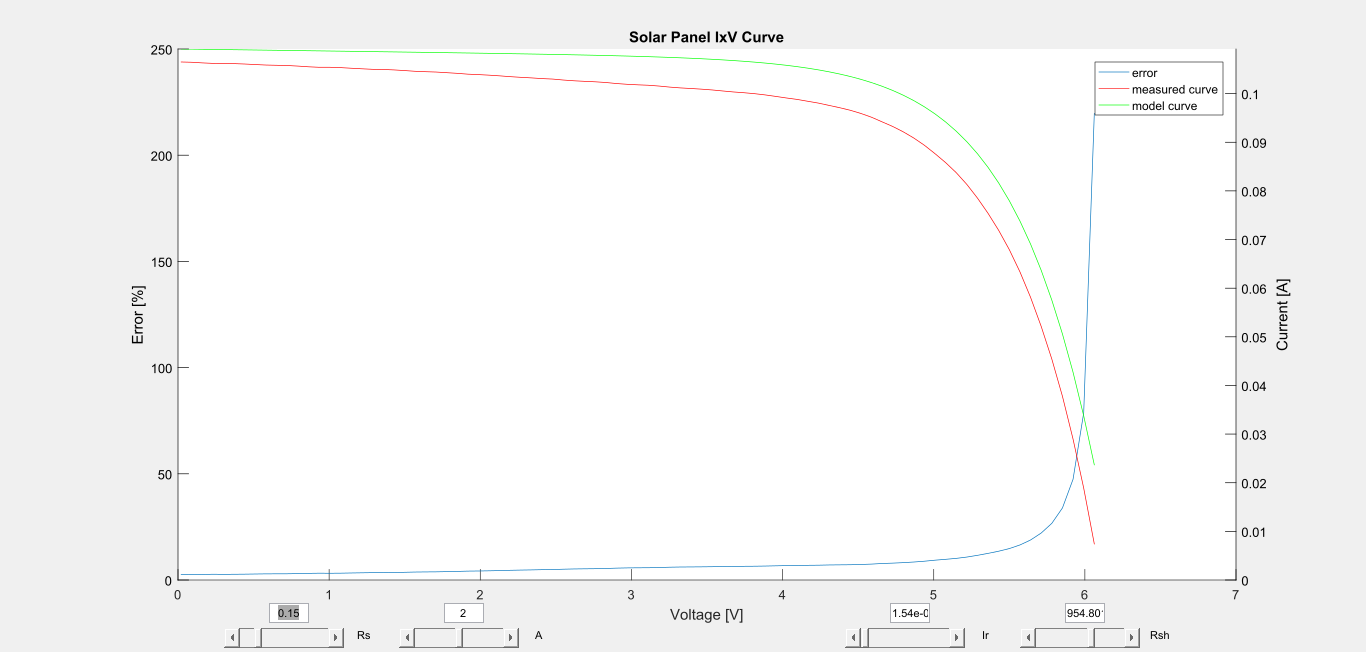
\includegraphics[scale=0.8]{figures/gui.pdf}
\caption{Interface Gráfica Para Ajuste da Curva}
\label{figura_interface_grafica}
\end{center}

\end{sidewaysfigure}

Os resultados estão na tabela \ref{parametros_modelo_painel_solar} e nas figuras \ref{figura_comparacao_150}, \ref{figura_comparacao_450} e \ref{figura_comparacao_700}. Foi possível manter o erro abaixo de \SI{5}{\percent} em toda a curva, exceto em regiões próximas a tensão de circuito aberto, as quais não são relevantes para este trabalho.

\begin{table}[!htpb]
\centering
\begin{tabular}{c c c c c}
\\ \hline
Irradiância [\SI{}{\watt\per\square\metre}] & R\textsubscript{s} [\SI{}{\ohm}] & R\textsubscript{p} [\SI{}{\ohm}] & I\textsubscript{o} [\SI{}{\nano\ampere}] & n \\ \hline \hline
500 & 0,15 & 599,602 & 154 & 2 \\
600 & 0,15 & 229,601 & 154 & 2 \\
700 & 0,15 & 140,801 & 154 & 2 \\ \hline
\end{tabular}
\caption{Parâmetros do Modelo do Painel Solar}
\label{parametros_modelo_painel_solar}
\end{table}

\pgfplotstableread[col sep = comma]{figures/VLDO-6A-model.csv}\solarPanelModelSix
\pgfplotstableread[col sep = comma]{figures/VLDO-6A.csv}\solarPanelMeasuredSix
\pgfplotstableread[col sep = comma]{figures/VLDO-7-5A-model.csv}\solarPanelModelSevenPointFive
\pgfplotstableread[col sep = comma]{figures/VLDO-7-5A.csv}\solarPanelMeasuredSevenPointFive
\pgfplotstableread[col sep = comma]{figures/VLDO-9A-model.csv}\solarPanelModelNine
\pgfplotstableread[col sep = comma]{figures/VLDO-9A.csv}\solarPanelMeasuredNine

\begin{figure}[!htpb]
\begin{minipage}{.5\textwidth}
\begin{center}
\begin{tikzpicture}[trim axis left, trim axis right]
\begin{axis}[xlabel = {V [\SI{}{\volt}]}, ylabel = {I [\SI{}{\ampere}]}, ymin = 0, scaled y ticks={base 10:2}, yticklabel style={/pgf/number format/fixed}, xtick distance=1, legend pos = south west, scale = 0.5, legend style = {font=\scriptsize}, scale only axis]
\addplot[mark = none, color = cyan] table[x index = {0}, y index = {1}]{\solarPanelModelSix};
\addplot[mark = none, color = red, dashed] table[x index = {0}, y index = {1}]{\solarPanelMeasuredSix};
\addlegendentry{Curva do Modelo}
\addlegendentry{Curva Medida}
\end{axis}
\end{tikzpicture}
\caption{Curvas para \SI[per-mode=symbol]{500}{\watt\per\square\meter}}
\label{figura_comparacao_150}
\end{center}
\end{minipage}
\begin{minipage}{.5\textwidth}
\begin{center}
\begin{tikzpicture}[trim axis left, trim axis right]
\begin{axis}[xlabel = {V [\SI{}{\volt}]}, ylabel = {I [\SI{}{\ampere}]}, ymin = 0, scaled y ticks={base 10:2}, yticklabel style={/pgf/number format/fixed}, xtick distance=1, legend pos = south west, legend style = {font=\scriptsize}, scale = 0.5, scale only axis]
\addplot[mark = none, color = cyan] table[x index = {0}, y index = {1}]{\solarPanelModelSevenPointFive};
\addplot[mark = none, color = red, dashed] table[x index = {0}, y index = {1}]{\solarPanelMeasuredSevenPointFive};
\addlegendentry{Curva do Modelo}
\addlegendentry{Curva Medida}
\end{axis}
\end{tikzpicture}
\caption{Curvas para \SI[per-mode=symbol]{600}{\watt\per\square\meter}}
\label{figura_comparacao_450}
\end{center}
\end{minipage}
\end{figure}

\begin{figure}[!htpb]
\begin{center}
\begin{tikzpicture}[trim axis left, trim axis right]
\begin{axis}[xlabel = {V [\SI{}{\volt}]}, ylabel = {I [\SI{}{\ampere}]}, ymin = 0, scaled y ticks={base 10:2}, yticklabel style={/pgf/number format/fixed}, xtick distance=1, legend pos = south west, legend style = {font=\scriptsize}, scale = 0.5, scale only axis]
\addplot[mark = none, color = cyan] table[x index = {0}, y index = {1}]{\solarPanelModelNine};
\addplot[mark = none, color = red, dashed] table[x index = {0}, y index = {1}]{\solarPanelMeasuredNine};
\addlegendentry{Curva do Modelo}
\addlegendentry{Curva Medida}
\end{axis}
\end{tikzpicture}
\caption{Curvas para \SI[per-mode=symbol]{700}{\watt\per\square\meter}}
\label{figura_comparacao_700}
\end{center}
\end{figure}

\section{\glsentryshort{mppt}}

Em geral, é muito custoso determinar pontos de operação possíveis em quantidade suficiente para controlar o sistema \gls{mppt} de forma satisfatória, portanto é necessário o emprego de algoritmos para determinar qual deve ser o ponto de operação em tempo real \cite{al2016}. Nas seguintes subseções serão descritos alguns destes algoritmos.

\subsection{\glsentrylong{peo}}

O algoritmo \gls{peo} funciona de acordo com o fluxograma da Figura \ref{fluxograma_algoritmo_peo}, no qual n é a iteração atual e P é a potência do painel. Primeiramente é gerada uma perturbação em sentido arbitrário no ponto de operação do painel. Em seguida, verifica-se se a potência entregue aumentou ou diminiu em relação a iteração anterior. Caso tenha aumentado mantém-se o sentido da perturbação aplicada, caso contrário o sentido é invertido. Desta forma o sistema irá caminhar na curva de potência até atingir o \gls{mpp}, sobre o qual ficará oscilando. Com isto evidencia-se um importante \textit{trade-off}: aumentar o passo da perturbação aumenta a velocidade com que o sistema atinge o \gls{mpp}, mas ao mesmo tempo faz com que a oscilação fique mais longe do \gls{mpp}, portanto é necessário encontrar um passo que satisfaça todos os requisitos de projeto.

A grande vantagem deste algoritmo é a sua simplicidade na implementação, que aliado com a sua alta eficiência quando implementado corretamente torna-o um dos algoritmos mais utilizados. A principal desvantagem é que este algoritmo demora a responder a variações grandes no ambiente. \cite{ngan2011}.

\begin{figure}[!htpb]
\begin{center}
\begin{tikzpicture}

\node [terminal, align = center](start){P(n) = 0 \\ P(n-1) = 0};
\node [process, below=of start, align = center](arbitrary_perturbation){Perturbação em Sentido Arbitrário};
\node [process, below=of arbitrary_perturbation, align = center](take_delta_P){\(\Delta\)P = P(n) - P(n-1)};
\node [decision, below=of take_delta_P, align = center](test_delta_P){\(\Delta\)P > 0?};
\node [process, left=of test_delta_P, align = center](keep_perturbation){Mantém o Sentido \\ da Perturbação};
\node [process, right=of test_delta_P, align = center](invert_perturbation){Inverte o Sentido \\ da Perturbação};
\path [line](start) -- (arbitrary_perturbation);
\path [line](arbitrary_perturbation) -- (take_delta_P);
\path [line](take_delta_P) -- (test_delta_P);
\path [line](test_delta_P) -- node[above]{sim} (keep_perturbation);
\path [line](test_delta_P) -- node[above]{não} (invert_perturbation);
\path [line](keep_perturbation) |- (take_delta_P);
\path [line](invert_perturbation) |- (take_delta_P);
\end{tikzpicture}

\end{center}
\caption{Fluxograma do algoritmo \glsentryshort{peo}}
\label{fluxograma_algoritmo_peo}
\end{figure}

\subsection{\glsentrylong{ci}}

O método da condutância incremental busca encontrar o \gls{mpp} utilizando-se do fato que a derivada da potência em relação à tensão no \gls{mpp} é nula, sendo este um ponto de máximo. Para fazer o rastreamento do \gls{mpp} é realizada a comparação da condutância incremental com a condutância instantânea \cite{ngan2011}. Para verificar como isto é possível vamos fazer a seguinte derivação, partindo da derivada da potência em relação a tensão:

\begin{equation} \label{eq:derivada_potencia_tensao}
\frac{dP}{dV} = \frac{d(IV)}{dV}
\end{equation}

Aplicando a regra do produto no lado direito equação \ref{eq:derivada_potencia_tensao} obtemos:
\begin{equation}
\begin{aligned}
\frac{dP}{dV} &= \frac{dI}{dV}\cdot V + \frac{dV}{dV}\cdot I \\
&= \frac{dI}{dV}\cdot V + I
\end{aligned}
\end{equation}

Pela curva PxV do painel podemos obter as seguintes afirmações:
\begin{gather*}
\begin{cases}
\frac{dI}{dV} = -\frac{I}{V} & \text{operando no \glsentryshort{mpp}} \\
\frac{dI}{dV} > -\frac{I}{V} & \text{operando à esquerda do \glsentryshort{mpp}} \\
\frac{dI}{dV} < -\frac{I}{V} & \text{operando à direita do \glsentryshort{mpp}}
\end{cases}
\end{gather*}

Assim, comparando a condutância incremental e a condutância instantânea é possível saber em qual posição da curva o painel está operando e tomar a atitude adequada. Este método apresenta resultados melhores que o \gls{peo} na maioria dos casos, principalmente quando as condições ambientais variam rapidamente, porém a complexidade dos cálculos realizados reduz um pouco seu uso \cite{tofoli2015}.

\subsection{\glsentrylong{aco}}

O algoritmo \gls{aco} é um algoritmo probabilístico usado para encontrar soluções globais para problemas não-lineares. Ele tenta imitar o comportamento de formigas em busca de comida para encontrar o melhor caminho em um grafo.

Quando formigas saem em busca de comida, inicialmente seu movimento é em direções aleatórias, até que seja encontrada comida. Quando isto acontece elas retornam à colônia, deixando feromônios no caminho, de forma que as próximas formigas irão seguir o mesmo caminho. Em caminhos mais longos os feromônios evaporam mais rápido, de forma que as formigas irão cada vez mais seguir os caminhos de menor distância \cite{dorigo2006}.

Para realizar \gls{mppt} com o algoritmo \gls{aco} primeiramente cada formiga do algoritmo é inicializada em um ponto aleatório de operação. Em seguida, o ferômonio é aumentado nos pontos de maior potência. A cada próxima iteração as formigas são inicializada em pontos distribuidos de forma aleatória em torno dos pontos com maior ferômonio. Assim é possível chegar ao \gls{mpp} \cite{jiang2013}.

Este algoritmo apresenta uma melhora em relação aos outros quando os paineis são operados parcialmente sob sombras, no qual a curva de potência apresenta vários máximos locais \cite{jiang2013}.

\subsection{Outros Algoritmos}

Em sistemas mais modernos outros tipos de algoritmos também são utilizados. Dentre eles podemos citar redes neurais \cite{elobaid2012}, algoritmos genéticos \cite{daraban2013}, entre outros.

Para este trabalho foi escolhido o algoritmo \gls{peo}, devido a sua eficiência aliada a sua grande simplicidade. O algoritmo foi implementado em um processador MSP430F6659. Devido a limitação no \textit{clock} deste processador, apenas trinta e dois passos de razão cíclica são possíveis.

\section{Conclusões}

Com o que foi desenvolvido e exposto neste capítulo foi possível entender o princípio básico de funcionamento das células solares. Além disso, foi apresentada uma interface gráfica para obter valores otimizados para os parâmetros do circuito equivalente das células. Também foi apresentada uma discussão sobre algoritmos \gls{mppt}, cada um com suas vantagens e desvantagens. Com isso os modelos necessários para uma simulação de painéis solares foram obtidos.